\chapter{OpenCL Driver for Zynq}
\label{ch4_OpenCL_Driver_for_Zynq}

We studied POCL software framework, which has performance portable kernel compiler. Also, we identified the necessary changes to add a new target device in POCL framework. In this chapter, we suggest a common OpenCL Driver for Zynq Platform using xillybus project. 

\section{Xillybus}
Xillybus project provides FPGA IP core design and necessary host drivers for Xilinx and Altera FPGA series. The Xillybus IP core designs are available in different licenses variants and the host drivers are open sourced for both Windows and Linux. Xillybus has an efficient DMA based solution for data transport between Linux or windows to FPGA device. It uses well known interface mechanism for both FPGA designers and host programmer developers. The design adopts interface as either of PCI Express or AXI. FPGA designers can develop the application logic that connects to the xillybus IP core through standard FIFO buffers. On the other hand, Programmer developer can use the file operations on pipes which is similar like a device file operation. They can control the data transfer using the file handler of a xillybus device file. Thus, it behaves like data streaming between FIFO buffers and the file handler opened by the application. Xillybus also provides an online tool to download the customized Xillybus IP core. We can customize parameters like expected bandwidth, number of streams etc., They estimated logic design consumption for Xilinx products are 110LUTs/Stream and 2500 LUTs with small number of RAMs  \cite{21}. Depending on host and FPGA capabilities, Xillybus can operate simultaneously up to 3.5GB/s in both directions. They also provide the source code for Linux drivers for xillybus interface. Xillybus has been used in applications like Data acquisition and playback, interfacing with required hardware, as a custom computer interface, coprocessing and more.

\section{Xillybus FPGA design interface}
Any application logic can be designed with xillybus IP. The xillybus IP core communicates data through standard FIFO buffer with the application logic. The FPGA designer has an advantage to choose the FIFO depth and the required interface with application logic. It is portable and efficient DMA based solution available both for Personal computers and Embedded Systems. The underlying communication is interfaced with either PCI Express or ARM--based AMBA bus (AXI3/AXI4). The example in the \ref{fig:1_XFI} \cite{22} gives a simplified block diagram for xillybus FPGA design interface for one data stream in each direction.
\begin{figure}[h]
    \centering
    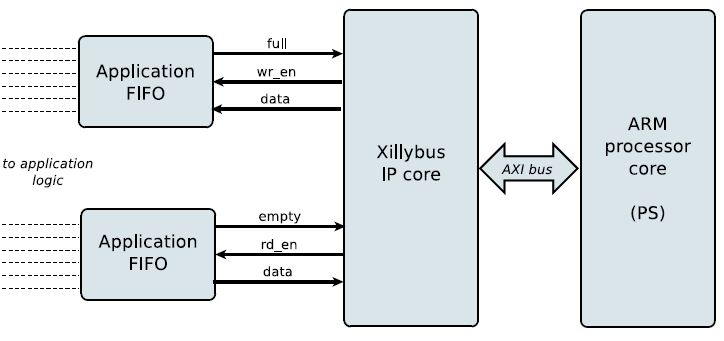
\includegraphics[width=1\textwidth]{xillybus_FPGA_Interface}
    \caption{Xillybus FPGA Interface}
    \label{fig:1_XFI}
\end{figure}

As shown in the example, when the data is written in lower FIFO buffer by application logic, the other end of the FIFO buffer senses the availability of data and transfers to the host. In the Processing System, it will be readable to the user--space software. Thus, the xillybus IP core setting relieves the FPGA designer from data traffic with the host. However, The IP manages to check the FIFOs ‘empty’ or ‘full’ signals and initiates data transfer accordingly. The xillybus is demonstrated with demo bundle which loopbacks the input and output direction FIFO buffers. These buffers in demo are configured with same clock. It cannot be used, when the FIFO are meant for cross clocking. Whenever a burst is started, xillybus IP core senses the empty or full signal and does not attempt to read from an empty buffer and to write in a full buffer. It serves all the connected buffer equally. FIFO buffers, which are getting filled fast, will be granted longer bursts. This simple arbitration gives efficient communication for the buffers that fill faster and follows low latency on FIFOs that receives little data.

\section{Xillybus Host application interface}

The Xillybus Linux host drivers generates named pipes to transfer data between FPGA and host. The Linux host drivers support any Xillybus IP configuration as it reads the required attributes from the xillybus IP core during initialization. The device file can be accessed at /dev/xillybus\_something. The device file can be opened, read and written to transfer and receive data as shown in the \ref{fig:2_HI} \cite{23}. It behaves like TCP/IP stream but on the other side it has FIFO in the FPGA. When the driver loads, FPGA is informed about the host's memory space addresses, where the DMA buffers are get allocated. The size of the buffers and number of buffers are retrieved during discovery process before allocation. Xillybus stream data can be categorized as synchronous and asynchronous based on a flag, which is fixed in FPGA’s logic. When the data flow is continuous, Asynchronous streams have better performance. During the custom IP core setting, the autoset internals can be turned off to select explicitly. The demo bundles provided, which has device files with xillybus\_write\_* and xillybus\_read\_* streams are asynchronous, while xillybus\_mem\_8 is synchronous.
\begin{figure}[h]
    \centering
    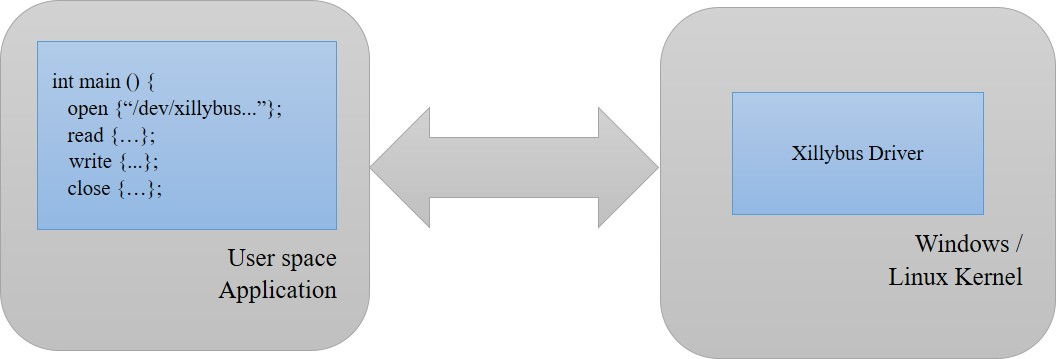
\includegraphics[width=1\textwidth]{host_interface}
    \caption{Host Interface}
    \label{fig:2_HI}
\end{figure}

For a continuous streaming process, when the hardware finished writing data to DMA buffers, it may send an interrupt to inform the software in the processing system to process the data. Similarly, the software after consuming the data, it informs the hardware to write the data again. Typically, this action is carried out using memory mapped register, where the hardware and software writes in the memory mapped register. Here, The Hardware and Software access DMA buffers in a round robin method. This technique creates the illusion of continuous data stream. Thus, the programmer can ignore the transport management when we have application data more than of DMA buffers size. 

\section{Xillybus as OpenCL Driver for Zynq Platform}
Xillybus is available for Zynq platform with customized Xillybus IP core and host Linux driver. The source code for the Linux environment are open sourced itself, but the xillybus IP core comes with variant licenses. Xillybus provides a Linux based distribution called Xillinux Distribution. It has demo drivers with host application examples. The key feature of using xillybus IP core is the design that allows the FPGA designer to connect their accelerator design or the application logic to the FIFO buffers without necessary management required for data transfer.

The motivation to develop Heterogeneous System Architecture with FPGAs is more promising in terms of power reduction, faster development and deployment. To avoid the difficulties in understanding about the underlying hardware, the parallel programming standards like OpenCL has taken over. Even though, to support a new target device for OpenCL Standard, we studied POCL software framework, which has modularized and performance portable kernel compiler for implementing OpenCL standard. POCL can be ported for Linux powered ARM--based Processing System. We propose an integration technique to use POCL framework and generalize OpenCL Implementation for Zynq Platform, which itself has a Processing System and Programmable Logic parts. To add a new device in POCL’s device layer, the first step should be the integration of OpenCL driver that can transfer the data between Processing System and the hardware device in PL. 

In POCL, ‘basic’ device layer can be customized with necessary integration for OpenCL drivers and the software package should be compiled on the platform or cross compiled to generate OpenCL Implemented library for Zynq Platform. Then using this library, host OpenCL application on Host can be build. The OpenCL drivers using xillybus host Linux drivers is targetable for any device in Programmable logic part of Zynq platform configured with xillybus IP core and application logic or accelerator design. Hence, The POCL’s basic device layer for write and read APIs can perform File operation on named pipes of xillybus IP to transfer the data between PS and PL. To increase the performance of data transfer, it is preferred to use asynchronous streaming configuration for xillybus core setting.

\section{Setting Xillinux Distribution}
The Xillinux Distribution is a development platform. This environment can be used for the custom logic in Programming Logic. Here, we discuss the steps to setup Xillinux distribution for Zedboard, which has ARM Cortex--A9 processor and a reconfigurable fabric. We must have two components to boot Xillinux distribution from a SD card. They are as follows,
\begin{itemize}\itemsep0em 
\item A FAT 32 filesystem in a boot partition that consists of bootloaders, bitstream of PL, and Linux kernel binary
\item An EXT4 root filesystem, which is mounted by Linux Operating system after loading Kernel.
\end{itemize}
We use the downloaded boot partition files, Xillinux image filesystem and the Xillybus project to boot the Zedboard with Xillinux distribution from xillybus website. 

\subsection{Unzipping the boot partition}
The xillybus project bundle for Zedboard, xillinux-eval-board-XXX.zip file is downloaded and extracted. It has following components with Verilog and VHDL files for main logic and block design files.
\begin{itemize}\itemsep0em 
\item verilog -- In src subdirectory, it contains the main logic for xillybus ip core in verilog.
\item vhdl -- In src subdirectory, the project file contains the main logic in user--editable VHDL source file.
\item cores -- Xillybus IP cores binaries are available, which are pre--compiled.
\item system -- It contains the directory for generating processor--related logic.
\item bootfiles -- This directory contains board--related binaries, which should be copied to /boot partition.
\item vivado--essentials – Contains processor--related and general--purpose logic files for use by Vivado.
\end{itemize}
The main interface file with xillybus IP core is xillydemo.v file, which is located in the ‘src’ subdirectory. These interface files can be edited to add their own data source and sinks. 

\subsection{Generating Bitstream}
Vivado design suite is a software suite developed by Xilinx for synthesis and HDL design analysis. To simplify the file structure, the bundle comes with the TCL script. The script creates a sub--directory with files as necessary. It is supported by Vivado 2014.4 or later version to run the TCL script. Following are the steps to generate bitstream for xillybus demo bundle.
\begin{enumerate}\itemsep0em 
\item Without opening new project, select Run TCL script from tools menu.
\item Browse for xillydemo--vivado.tcl script, which can be located at verilog/ subdirectory.
\item After series of events, project created message can be found in TCL console tab at Vivado's window as shown below.
	\lstinputlisting[firstline=23, lastline=23, frame=none, basicstyle=\fontsize{11}{11}\selectfont\ttfamily, backgroundcolor=\color{gainsboro}]{code_snippet.txt}
\item After Project creation, Implementation should be run successfully. Bitstream can be created by selecting generate bitstream option on the flow navigator bar.
\item	The generated bitstream can be found at vivado/xillydemo.runs/impl\_1/
\end{enumerate}

\subsection{Loading the Linux Image}
The main task in this section is to load the system Image file to the (Micro) SD device. It can be accomplished in a Desktop environment using windows or Linux based operating system. The image file downloaded under the name xillinux.img.gz is extracted using gzip compression technique. This image contains two major partitions called boot and root. Boot partition is populated as FAT32 filesystem and it is placed with initial bootloaders and kernel binaries, while the root partition is ext4 filesystem for Linux root file system. Writing the downloaded image requires additional software and the previous content in the SD device will be deleted. We prefer to use Linux desktop environment to load the image. The following steps will write the image to SD device.
\begin{enumerate}\itemsep0em 
	\item Identifying the connected SD device name using system main log file. The log file can be found at /var/log/messages or /var/log/syslog or using dmesg linux command
	\lstinputlisting[firstline=1, lastline=8, frame=none, basicstyle=\fontsize{8}{8}\selectfont\ttfamily, backgroundcolor=\color{gainsboro}]{code_snippet.txt}
	\item The kernel will assign the name to the connected SD device, which should be like “sda” or “mmcblk”.
	\item The Downloaded image file can be uncompressed using gunzip.
	\lstinputlisting[firstline=10, lastline=10, frame=none, basicstyle=\fontsize{11}{11}\selectfont\ttfamily, backgroundcolor=\color{gainsboro}]{code_snippet.txt}
	\item We can copy the image to SD card using dd command. In the command, we should point out the correct SD device name from step 2.
	\lstinputlisting[firstline=12, lastline=12, frame=none, basicstyle=\fontsize{11}{11}\selectfont\ttfamily, backgroundcolor=\color{gainsboro}]{code_snippet.txt}
	\item After writing into SD device, we compare the content in SD device and the image file using cmp command. If we get a EOF message, the comparison is correct or If we didn’t get any message, a regular file is generated instead of writing.
	\lstinputlisting[firstline=14, lastline=15, frame=none, basicstyle=\fontsize{11}{11}\selectfont\ttfamily, backgroundcolor=\color{gainsboro}]{code_snippet.txt}
	\item The SD card device can be removed and connected back to Desktop.
	\item Copy the devicetree.dtb and boot.bin from boot partition bundle in bootfiles/ subdirectory into SD card’s boot partition. 
	\item The PL configuration bitstream, which was generated by previous section should be copied to the boot partition of SD card.
	\item Check for the following files in the boot partition.
	\begin{enumerate}\itemsep0em 
		\item uImage -- Board independent Linux Kernel file
		\item boot.bin -- The initial bootloader that has initial processor initialization and u--boot utility.
		\item devicetree.dtb -- This file is a input to the Linux kernel, which has a hardware information. It is called device tree blob.
		\item xillydemo.bit -- The Programmable Logic configuration file has an Xillybus IP core with FIFO loopback.
	\end{enumerate}
\end{enumerate}

\subsection{Booting up}
The basic peripheral connection should be a USB to UART connection between Desktop and Zedboard for debugging. The default UART setting in Zedboard is 115200 baud, 8 data bits and 1 stop bit with no flow control mechanism.  In the desktop environment, we can use Teraterm for windows or Minicom for Ubuntu Distribution with the latter UART configuration for serial port connection with Zedboard. Also, the board should be configured with the following jumper settings to change the boot source to (Micro) SD Card.
\begin{itemize}\itemsep0em 
	\item A jumper is installed in JP2 to supply 5V to USB device.
	\item JP10 and JP9 are changed from GND to 3V3 position, the other three jumpers in that row are connected to GND.
	\item A jumper is installed at JP6.
\end{itemize}

The system is powered on and booted with default environmental variables. As the root filesystem image is kept small for easy copying, it is recommended to resize the file system to the maximum. The following steps will resize the root partition with SD card’s full capacity.
\begin{enumerate}\itemsep0em 
	\item Initially, the current allocated size of the filesystem is identified using df command.
	\lstinputlisting[firstline=17, lastline=17, frame=none, basicstyle=\fontsize{11}{11}\selectfont\ttfamily, backgroundcolor=\color{gainsboro}]{code_snippet.txt}
	\item Fdisk utility is used to recreate the root filesystem. Following are the options available in fdisk.
	\begin{itemize}\itemsep0em 
	\item d [ENTER] -- Delete partition
	\item n [ENTER] -- Create a new partition
	\item w [ENTER] -- Save and quit.
	\end{itemize}
	\item By passing SD card device name to fdisk command, the second partition is deleted and a new primary partition is created with all default values. 
	\lstinputlisting[firstline=19, lastline=19, frame=none, basicstyle=\fontsize{11}{11}\selectfont\ttfamily, backgroundcolor=\color{gainsboro}]{code_snippet.txt}
	\item After rebooting the system, the filesystem can be resized using following command.
	\lstinputlisting[firstline=21, lastline=21, frame=none, basicstyle=\fontsize{11}{11}\selectfont\ttfamily, backgroundcolor=\color{gainsboro}]{code_snippet.txt}
\end{enumerate}